%  Pt1.tex
% !TeX spellcheck = en_GB
% !TeX root = ProjectRiskManagement.tex

\section{Approaches to Uncertainty and Underlying Complexity Management - 1200}

Introduction to risk and opportunity, underlying complexity. 

Challenge of traditional view of risk.

%Project life cycle introduction.
A traditional view of the asset/change lifecycle is a useful indicator of the scope of a project and the potential activities required.
However, a more detailed outlook is often required.
Both views are shown in figure \ref{Figure:Project_Lifecycle}.
The 12-stage lifecycle is shown as a subset of the 4-stage traditional view.

% execution and delivery strategy shaping phase of a project's life cycle
This paper focusses on PUMPs within the context of the Execution and Delivery (E\&D) stage.

\begin{figure}[!h]
  \centering
    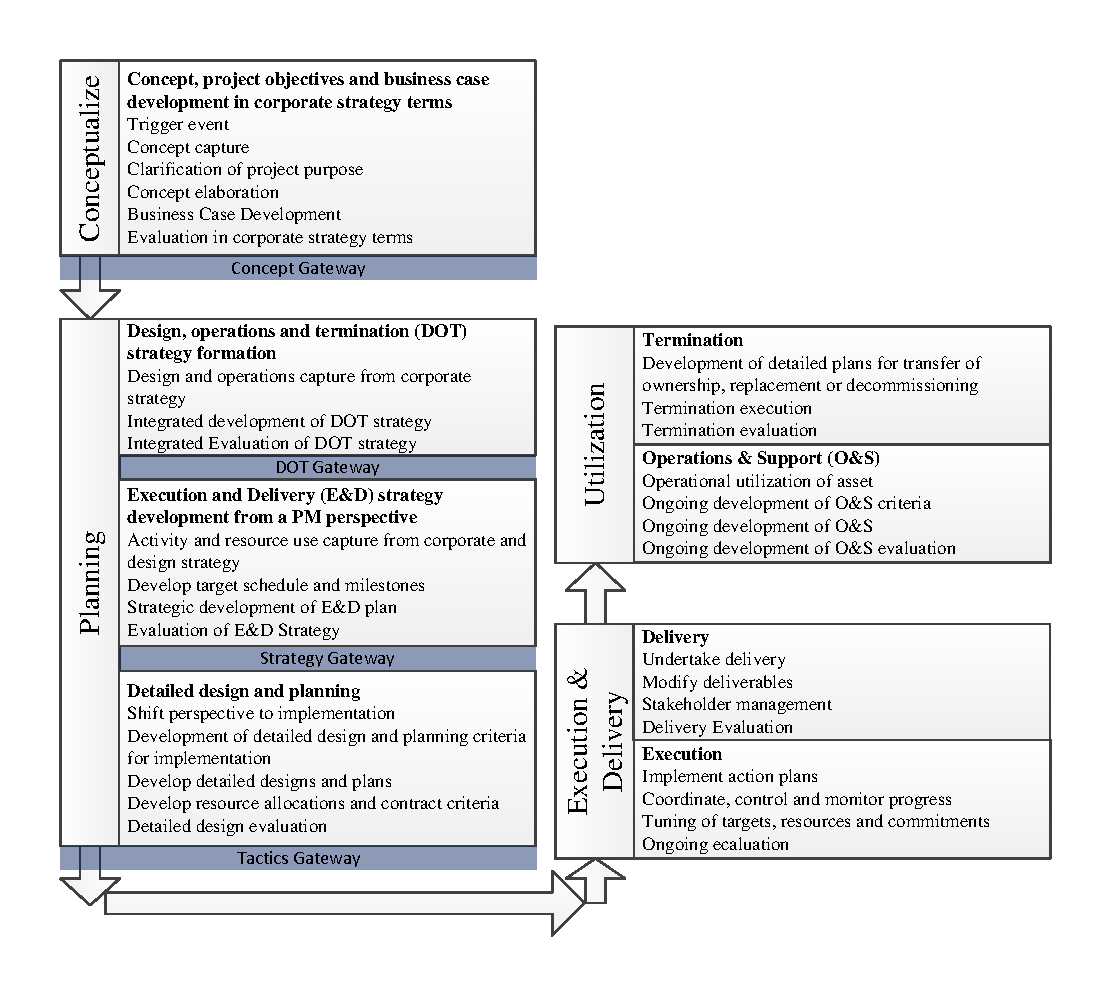
\includegraphics[width = \textwidth]{./Figures/ProjectLifecycleDetailedCurve.pdf} 
\caption{12-stage project lifecycle - adapted from \cite{chapman}}
\label{Figure:Project_Lifecycle}
\end{figure}

\subsection{The PUMP Process}
%Explain concisely in your own words what you believe are the key overall features of a PUMP approach to project risk management in the execution and delivery strategy shaping phase of a project’s lifecycle. Compare these features with the PMI PIMBOK approach or any other form of common practice you are familiar with if you find this helpful, but focus on the PUMP approach. Use examples to illustrate your discussion if you wish, but concentrate on concepts and principles. This will be a largely descriptive summary of your interpretation of the lectures and associated reading. It will demonstrate your grasp of the central core of the unit’s material as a whole, and should be approached with a view to demonstrating this understanding..

\subsection{Contrast with Other Risk Management Processes}
Contrast with PUMP and PMI PMBOK and others.

\subsection{The Clarity Efficient Approach}
Summarise that PUMPS offer a higher level of clarity for the project as a whole rather than 


1200words.